\section{Nuovi risultati}

\subsection{Dataset originale}

\subsubsection{Dataset completo}

I nuovi dati hanno portato alla seguente distribuzione dei dati (qui di seguito visualizzata):
\begin{figure}[H]
    \centering
    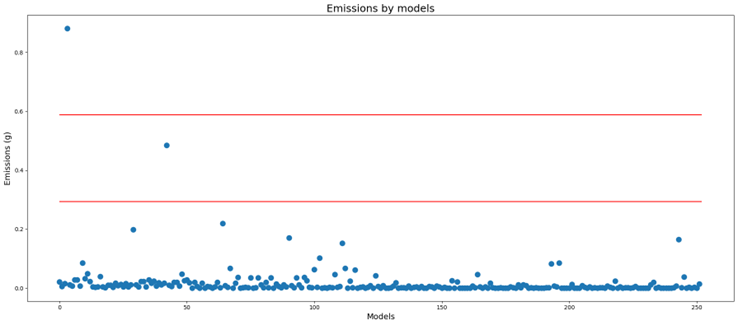
\includegraphics[scale=1.25]{images/nuova-situazione.png}
\end{figure}

Come è possibile notare, i nuovi esperimenti hanno portato a un'ulteriore sbilanciamento nel dataset, in quanto tutti gli esperimenti con DGCF svettano sui risultati degli altri modelli.

Questo si riflette nei risultati ottenuti dai modelli di regressione

\begin{table}[H]
    \centering
    \begin{tabular}{|>{\centering\arraybackslash}m{5cm}|c|c|c|c|}
        \hline
        \textbf{Regressor} & \textbf{MAE} & \textbf{RMSE} & \textbf{MSLE} \\ [10pt]
        \hline
        SVR & 0.0995056 & 0.0161732 & 0.0111161 \\ [10pt]
        \hline
        Decision Tree & 0.0201826 & 0.0037623 & 0.0021361 \\ [10pt]
        \hline
        Random Forest & 0.0236930 & 0.0078052 & 0.0039711 \\ [10pt]
        \hline
        AdaBoost & 0.0311916 & 0.0053061 & 0.0029177 \\ [10pt]
        \hline
    \end{tabular}
    \caption*{Risultati ottenuti}
    \label{tab:results}
\end{table}

//TODO: aggiungere le nuove learning curve se necessario

\subsubsection{Dataset Azure}

\noindent Una possibile soluzione è stata quella di eliminare tutti i risultati non prodotti sulla macchina Azure. Le emissioni risultato ancora sbilanciate ma si è riscontrato un leggero miglioramento nei risultati dei modelli di regressione

\begin{figure}[H]
    \centering
    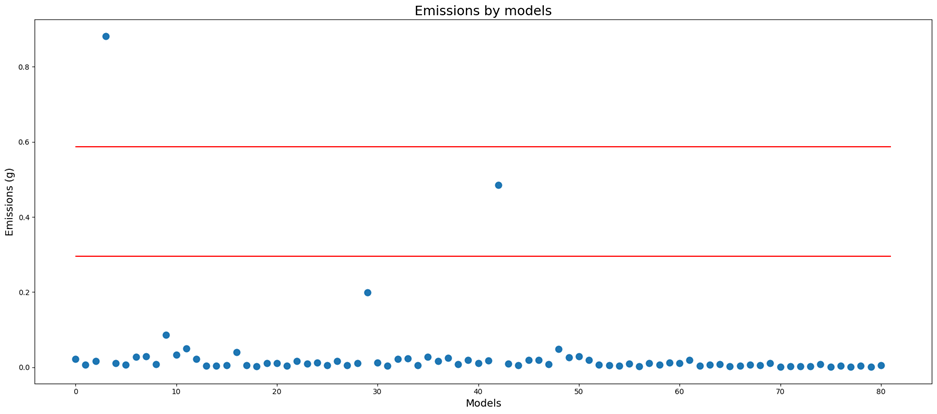
\includegraphics[scale=1.25]{images/nuova-situazione2.png}
\end{figure}



\begin{table}[H]
    \centering
    \begin{tabular}{|>{\centering\arraybackslash}m{5cm}|c|c|c|c|}
        \hline
        \textbf{Regressor} & \textbf{MAE} & \textbf{RMSE} & \textbf{MSLE} \\ [10pt]
        \hline
        SVR & 0.0923003 & 0.0085932 & 0.0076811 \\ [10pt]
        \hline
        Decision Tree & 0.0165181 & 0.0033569 & 0.0019016 \\ [10pt]
        \hline
        Random Forest & 0.0144149 & 0.0007829 & 0.0005558 \\ [10pt]
        \hline
        AdaBoost & 0.0221310 & 0.0035251 & 0.0020638 \\ [10pt]
        \hline
    \end{tabular}
    \caption*{Risultati ottenuti}
    \label{tab:results}
\end{table}

//TODO: aggiungere le nuove learning curve se necessario



\subsection{Dataset ridotto}

Per provare a migliorare ancor di più le performance dei modelli di regressione, si è deciso di eliminare tutti gli outlier dal dataset(in questo caso le emissioni più alte). In particolare si sono eliminate 11 emissioni dal dataset completo e 5 dal dataset AZURE.

\subsubsection{Dataset completo}

\begin{figure}[H]
    \centering
    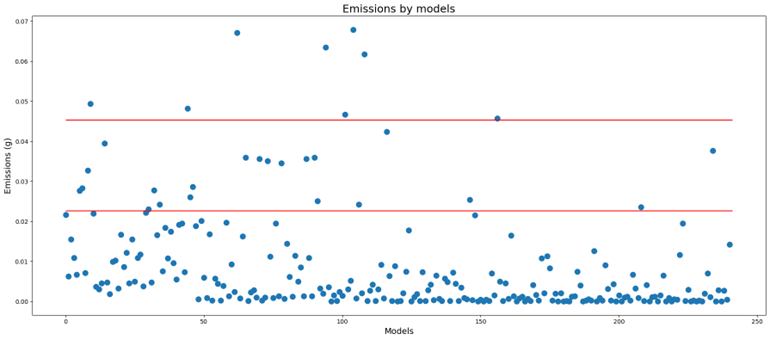
\includegraphics[scale=1.25]{images/nuova-situazione-ridotto.png}
\end{figure}

E' possibile notare un miglior bilanciamento delle emissioni. Per quanto riguarda i modelli, sono stati eseguti addestramenti con diversi split tra training e test set

\textbf{Slit 50/50}


\begin{table}[H]
    \centering
    \begin{tabular}{|>{\centering\arraybackslash}m{5cm}|c|c|c|c|}
        \hline
        \textbf{Regressor} & \textbf{MAE} & \textbf{RMSE} & \textbf{MSLE} \\ [10pt]
        \hline
        SVR & 0.026350 & 0.0008080 & 0.0007787 \\ [10pt]
        \hline
        Decision Tree & 0.0091483 & 0.0003243 & 0.0003048 \\ [10pt]
        \hline
        Random Forest & 0.0073434 & 0.0001388 & 0.00013121 \\ [10pt]
        \hline
        AdaBoost & 0.0115256 & 0.0003340 & 0.0003147 \\ [10pt]
        \hline
    \end{tabular}
    \caption*{Risultati ottenuti}
    \label{tab:results}
\end{table}

//TODO: aggiungere le nuove learning curve se necessario

\textbf{Split 60/40}


\begin{table}[H]
    \centering
    \begin{tabular}{|>{\centering\arraybackslash}m{5cm}|c|c|c|c|}
        \hline
        \textbf{Regressor} & \textbf{MAE} & \textbf{RMSE} & \textbf{MSLE} \\ [10pt]
        \hline
        SVR & 0.0264396 & 0.0007823 & 0.000754 \\ [10pt]
        \hline
        Decision Tree & 0.0079836 & 0.0001961 & 0.0001866 \\ [10pt]
        \hline
        Random Forest & 0.0069729 & 0.0001164 & 0.0001116 \\ [10pt]
        \hline
        AdaBoost & 0.0081044 & 0.0001324 & 0.0001269 \\ [10pt]
        \hline
    \end{tabular}
    \caption*{Risultati ottenuti}
    \label{tab:results}
\end{table}

//TODO: aggiungere le nuove learning curve se necessario

\textbf{Split 70/30}


\begin{table}[H]
    \centering
    \begin{tabular}{|>{\centering\arraybackslash}m{5cm}|c|c|c|c|}
        \hline
        \textbf{Regressor} & \textbf{MAE} & \textbf{RMSE} & \textbf{MSLE} \\ [10pt]
        \hline
        SVR & 0.02635137 & 0.0007884 & 0.0007602 \\ [10pt]
        \hline
        Decision Tree & 0.0072258 & 0.0001427 & 0.0001372 \\ [10pt]
        \hline
        Random Forest & 0.0068948 & 0.0001102 & 0.0001059 \\ [10pt]
        \hline
        AdaBoost & 0.0076783 & 0.0001130 & 0.0001089 \\ [10pt]
        \hline
    \end{tabular}
    \caption*{Risultati ottenuti}
    \label{tab:results}
\end{table}

//TODO: aggiungere le nuove learning curve se necessario


\textbf{Split 80/20}


\begin{table}[H]
    \centering
    \begin{tabular}{|>{\centering\arraybackslash}m{5cm}|c|c|c|c|}
        \hline
        \textbf{Regressor} & \textbf{MAE} & \textbf{RMSE} & \textbf{MSLE} \\ [10pt]
        \hline
        SVR & 0.0270399 & 0.0008109 & 0.0007820 \\ [10pt]
        \hline
        Decision Tree & 0.0067696 & 0.0001287 & 0.0001236 \\ [10pt]
        \hline
        Random Forest & 0.0063234 & 0.0001004 & 0.0000967 \\ [10pt]
        \hline
        AdaBoost & 0.0081434 & 0.0001208 & 0.0001167 \\ [10pt]
        \hline
    \end{tabular}
    \caption*{Risultati ottenuti}
    \label{tab:results}
\end{table}

//TODO: aggiungere le nuove learning curve se necessario



\textbf{Split 90/10}


\begin{table}[H]
    \centering
    \begin{tabular}{|>{\centering\arraybackslash}m{5cm}|c|c|c|c|}
        \hline
        \textbf{Regressor} & \textbf{MAE} & \textbf{RMSE} & \textbf{MSLE} \\ [10pt]
        \hline
        SVR & 0.0266539 & 0.0007763 & 0.0007483 \\ [10pt]
        \hline
        Decision Tree & 0.0056915 & 0.0000799 & 0.0000774 \\ [10pt]
        \hline
        Random Forest & 0.0051378 & 0.0000524 & 0.0000509 \\ [10pt]
        \hline
        AdaBoost & 0.0073941 & 0.00000991 & 0.0000961 \\ [10pt]
        \hline
    \end{tabular}
    \caption*{Risultati ottenuti}
    \label{tab:results}
\end{table}


TODO: aggiungere le nuove learning curve se necessario



\textbf{Conclusioni}

Come si può notare in generale la riduzione del dataset ha portato a miglioramenti. Per quanto riguarda i diversi split si può notare che alcuni modelli performano meglio con alcuni split, altri modelli con altri


\subsubsection{Dataset AZURE}

\begin{figure}[H]
    \centering
    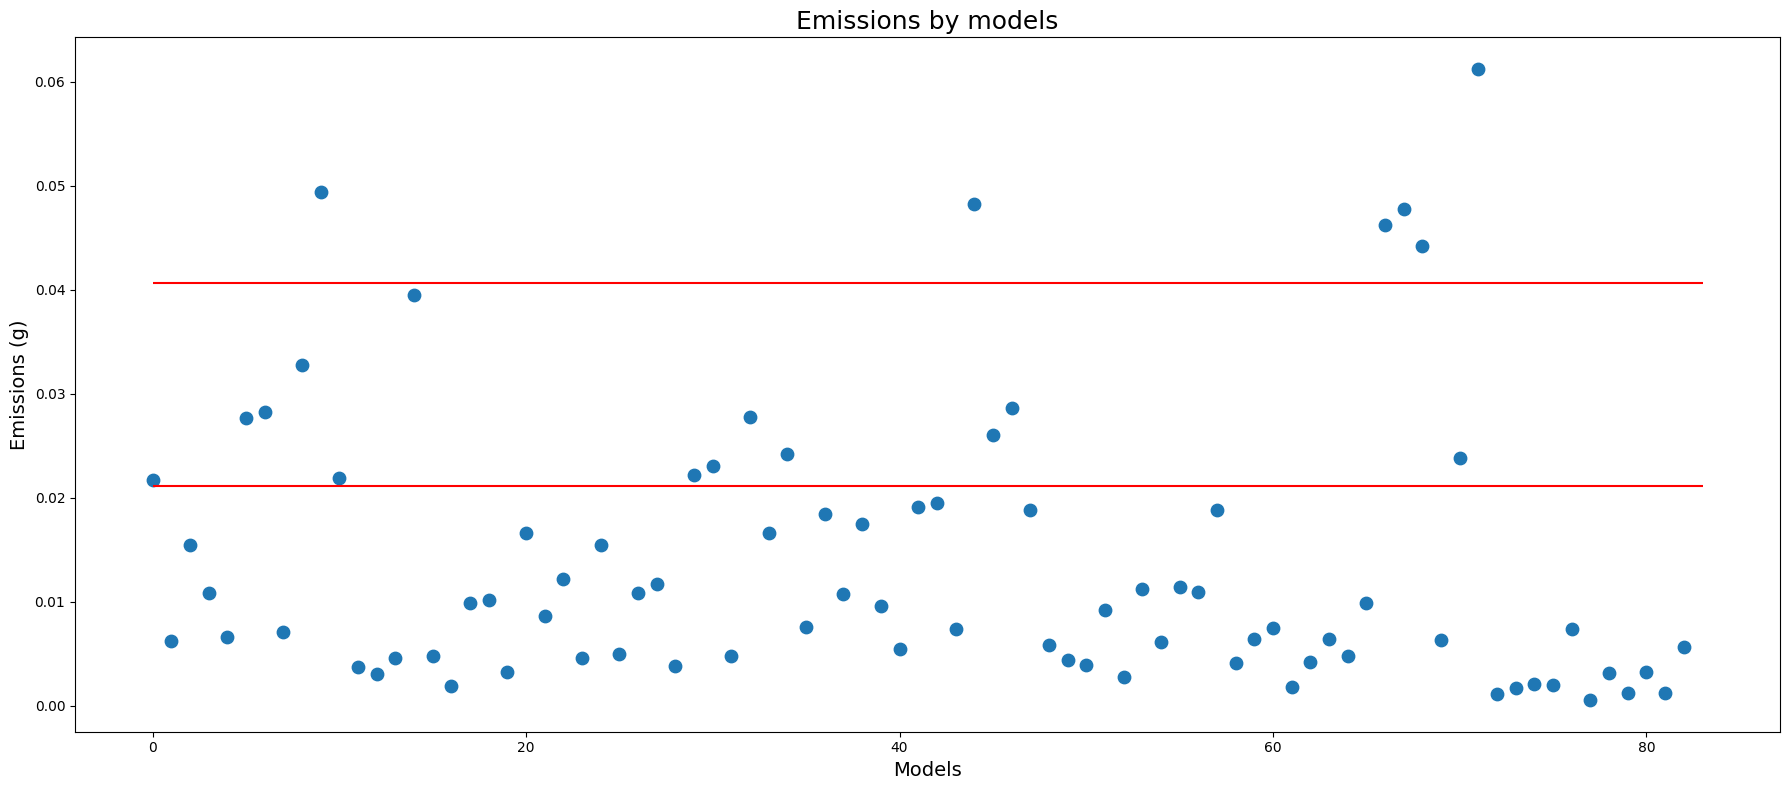
\includegraphics[scale=1.25]{images/nuova-situazione2-ridotto.png}
\end{figure}


E’ possibile notare un miglior bilanciamento delle emissioni. Per quanto riguarda i modelli,
sono stati eseguti addestramenti con diversi split tra training e test set


\textbf{Slit 50/50}


\begin{table}[H]
    \centering
    \begin{tabular}{|>{\centering\arraybackslash}m{5cm}|c|c|c|c|}
        \hline
        \textbf{Regressor} & \textbf{MAE} & \textbf{RMSE} & \textbf{MSLE} \\ [10pt]
        \hline
        SVR & 0.0148003 & 0.0002638 & 0.0002559 \\ [10pt]
        \hline
        Decision Tree & 0.0066692 & 0.0001030 & 0.0000987 \\ [10pt]
        \hline
        Random Forest & 0.0056723 & 0.0000667 & 0.0000644 \\ [10pt]
        \hline
        AdaBoost & 0.0070703 & 0.0001008 & 0.0000975 \\ [10pt]
        \hline
    \end{tabular}
    \caption*{Risultati ottenuti}
    \label{tab:results}
\end{table}

//TODO: aggiungere le nuove learning curve se necessario

\textbf{Split 60/40}


\begin{table}[H]
    \centering
    \begin{tabular}{|>{\centering\arraybackslash}m{5cm}|c|c|c|c|}
        \hline
        \textbf{Regressor} & \textbf{MAE} & \textbf{RMSE} & \textbf{MSLE} \\ [10pt]
        \hline
        SVR & 0.0148974 & 0.000269 & 0.0002609 \\ [10pt]
        \hline
        Decision Tree & 0.0071797 & 0.0001293 & 0.00001239 \\ [10pt]
        \hline
        Random Forest & 0.0049437 & 0.0000621 & 0.0000598 \\ [10pt]
        \hline
        AdaBoost & 0.0059144 & 0.0000805 & 0.0000775 \\ [10pt]
        \hline
    \end{tabular}
    \caption*{Risultati ottenuti}
    \label{tab:results}
\end{table}

//TODO: aggiungere le nuove learning curve se necessario

\textbf{Split 70/30}


\begin{table}[H]
    \centering
    \begin{tabular}{|>{\centering\arraybackslash}m{5cm}|c|c|c|c|}
        \hline
        \textbf{Regressor} & \textbf{MAE} & \textbf{RMSE} & \textbf{MSLE} \\ [10pt]
        \hline
        SVR & 0.0145669 & 0.0002622 & 0.0002543 \\ [10pt]
        \hline
        Decision Tree & 0.0059280 & 0.0000885 & 0.0000851 \\ [10pt]
        \hline
        Random Forest & 0.0057711 & 0.0000790 & 0.000076 \\ [10pt]
        \hline
        AdaBoost & 0.0065205 & 0.0000858 & 0.0000827 \\ [10pt]
        \hline
    \end{tabular}
    \caption*{Risultati ottenuti}
    \label{tab:results}
\end{table}

//TODO: aggiungere le nuove learning curve se necessario


\textbf{Split 80/20}


\begin{table}[H]
    \centering
    \begin{tabular}{|>{\centering\arraybackslash}m{5cm}|c|c|c|c|}
        \hline
        \textbf{Regressor} & \textbf{MAE} & \textbf{RMSE} & \textbf{MSLE} \\ [10pt]
        \hline
        SVR & 0.0137841 & 0.0002431 & 0.0002356 \\ [10pt]
        \hline
        Decision Tree & 0.0070346 & 0.0001177 & 0.0001133 \\ [10pt]
        \hline
        Random Forest & 0.0061398 & 0.0001047 & 0.0001007 \\ [10pt]
        \hline
        AdaBoost & 0.0073228 & 0.0001225 & 0.0001181 \\ [10pt]
        \hline
    \end{tabular}
    \caption*{Risultati ottenuti}
    \label{tab:results}
\end{table}

//TODO: aggiungere le nuove learning curve se necessario



\textbf{Split 90/10}

\begin{table}[H]
    \centering
    \begin{tabular}{|>{\centering\arraybackslash}m{5cm}|c|c|c|c|}
        \hline
        \textbf{Regressor} & \textbf{MAE} & \textbf{RMSE} & \textbf{MSLE} \\ [10pt]
        \hline
        SVR & 0.0193509 & 0.0003821 & 0.0003712 \\ [10pt]
        \hline
        Decision Tree & 0.0055465 & 0.0000506 & 0.0000494 \\ [10pt]
        \hline
        Random Forest & 0.0032249 & 0.000021 & 0.0000207 \\ [10pt]
        \hline
        AdaBoost & 0.0050706 & 0.0000415 & 0.00000406 \\ [10pt]
        \hline
    \end{tabular}
    \caption*{Risultati ottenuti}
    \label{tab:results}
\end{table}


TODO: aggiungere le nuove learning curve se necessario



\textbf{Conclusioni}

Come si può notare in generale la riduzione del dataset ha portato a miglioramenti. Per quanto riguarda i diversi split si può notare che alcuni modelli performano meglio con alcuni split, altri modelli con altri


\subsubsection{Dataset AZURE}

\begin{figure}[H]
    \centering
    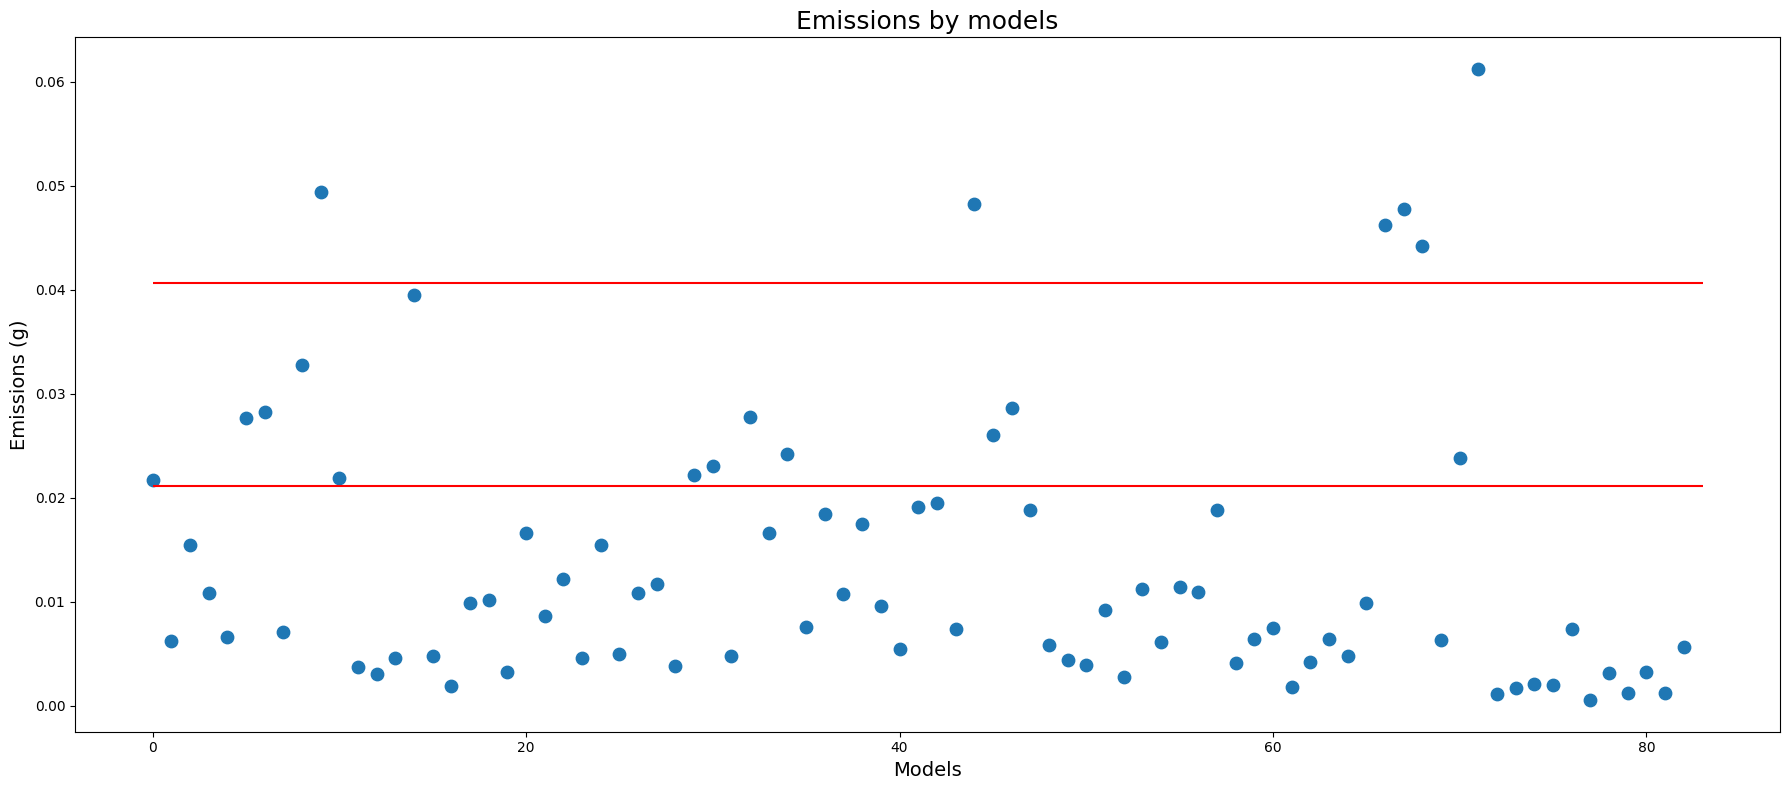
\includegraphics[scale=1.25]{images/nuova-situazione2-ridotto.png}
\end{figure}